\documentclass[11pt]{article}
\usepackage{graphicx}
\usepackage{url}
\usepackage[small]{caption2}
\renewcommand{\baselinestretch}{1.0}
\title{Project 1}
\author{Knut Halvor Skrede}
\setlength{\parindent}{0pt}
\setlength{\parskip}{2ex} 
\begin{document}
\maketitle
\clearpage

\section*{Part A)}

\subsection*{Code description} %1. A clear, concise description of your EA code in text and a few diagrams (2 points).

The code for the EA is written in c++. It consists of 4 classes; 
BasicEA, Strategies, Population and Individual.
The BasicEA class implements the main loop. This loop goes through
the main functionality of the Population class.
The main functionality of the population class is to call the
member functions implemented in the Individual class using the
\begin{figure}[ht]
\begin{center}
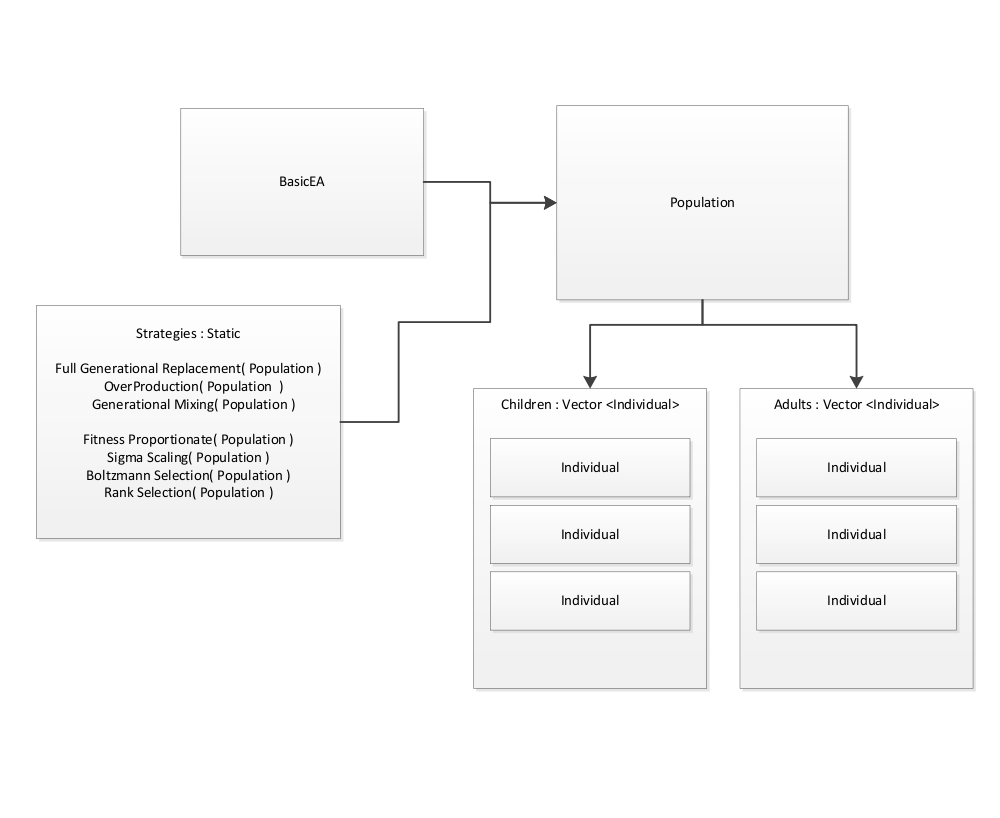
\includegraphics[width=\textwidth]{images/classes.png}
\end{center}
\caption{Simple layout of classes}
\label{fig:classes}
\end{figure}
strategies implemented in the Strategies class. See figure \ref{fig:classes}
for a simple layout. The Population class also implements functionality
to collect statistics and other helpfull information.

The program takes the following parameters as arguments:
\begin{enumerate}
\renewcommand{\theenumii}{\arabic{enumii}}
\item Size of child pool [integer]
\item Size of adult pool [integer]
\item number of generations [integer]
\item mutation rate [float between 0.0 and 1.0]
\item crossover rate [float between 0.0 and 1.0]
\item selection protocol [integer between 1 and 3]
   \begin{enumerate}
   \item Full Generational replacement (parameter 1 and 2 must be equal)
   \item Over-production (parameter 1 must be larger than paramter 2)
   \item Generational-mixing
   \end{enumerate}
\item selection strategy [integer between 1 and 4]
   \begin{enumerate}
   \item Fitness proportionate
   \item Sigma scaling
   \item Boltzmann selection
   \item Rank selection
   \item Tournament selection
   \end{enumerate}
\item Elitism [integer]
\item If boltzmann selection: Temperature [float greater than 0]\\
      If tournament selection: Tournament size [integer greater than 2 and less than halv the size of adult pool]

\end{enumerate}

\subsection*{Genotype representation}

The genotype is represented as an array of 40 boolean values.

\subsection*{Developmental method}

The developmental method converts the genotype (array of 40 boolean values) into
a phenotype (array of 10 integers between 0 and 15.)

\subsection*{Fitness evaluation}

The Individuals class implements it's own fitness evaluation function. Here
it is simply the sum of all integers in the phenotype.

\subsection*{Selection protocols}

The selection mechanisms for parent selection fills the child pool with
a number of children, provided as an argument to the application.
The selection protocols are then responsible for choosing which of the 
children become adults. All the suggested selection protocols (Full generational 
replacement, Over-production and Generational Mixing) are implemented
in the Strategies class.

\subsection*{Selection mechanisms}

\subsubsection*{Tournament selection}

When using tournament selection, and a crossover is to be performed, two
tournaments are arranged to find both parents. Therefore, the size of the
tournament groups must be half of the size of the adult pool.

\subsubsection*{Other selection mechanisms}

All the other selection mechanisms are implemented as a roulette wheel, where
the expected values are calculated according to the respective methods (Fitness proportionate,
Sigma scaling, Boltzmann selection or Rank selection.)

\subsection*{Genetic operators}

\subsubsection*{Crossover}

The crossover functionality was implemented as a random bitmask that 
chooses which genotypes come from each parent. And by remembering that
bitmask, and by always producing two children, I can guarantee that the 
crossover will reprecent the entire genotype to the next generation.

\subsubsection*{Mutation}

Mutation is implemented as a function that flips a random bit in the genotype.
All children has a probability equal to the mutation rate parameter to be
mutated. 

\subsubsection*{Elitism}

Elitism is implemented such that a parameter (elitism) chooses how many
of the best individuals are to be cloned into the child pool. However, elite 
individuals have to be selected according to the selection mechanism in order
to become adults, and since I mutate across the entire child pool after reproduction, 
elite individuals may be mutated.

\subsection*{Code modularity} %2. A justification of your code’s modularity and reusability. You should describe how easy it is for your code to incorporate new phenotypes, genotypes, genetic operators and selection mechanisms as may be needed to handle new problems. (1 point).

All the main strategies and protocols are implemented in the Strategies class and
uses the functions implemented in the Population and Individual classes.
This way, I just have to change the Individual class to adapt problems to the
BasicEA and I only have to alter the Strategies class to alter the 
main strategies and protocols.

\subsection*{Performance analysis} %3. An analysis of the performance of your EA on a 40-bit One-Max problem where the adult selection protocol is full-generational replacement and the parent selection mechanism is fitness-proportionate. First run the problem using various population sizes until you find the approximately minimal size that allows One-Max solutions to be consistently found in under 100 generations. Then, using only that population size, experiment with different values for the crossover and mutation rates. Use fitness plots to show the different results. Make a statement as to what the best choices are for these parameters in your runs. (2 points)

\begin{figure}[ht]
\begin{center}
\mbox{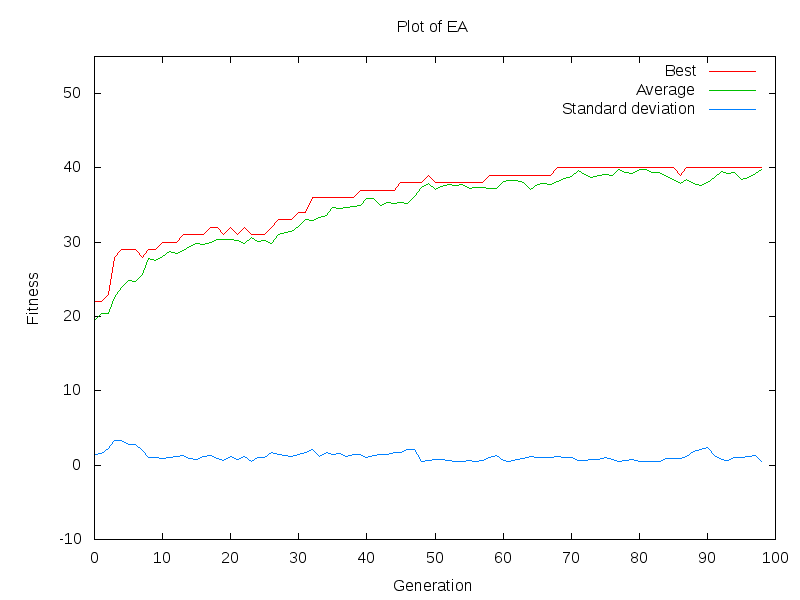
\includegraphics[width=0.49\textwidth]{images/11.png}}
\mbox{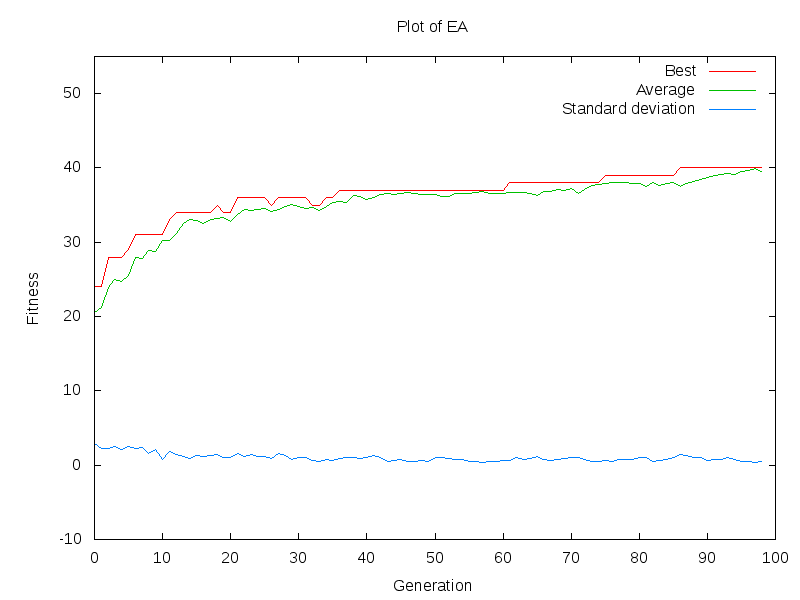
\includegraphics[width=0.49\textwidth]{images/12.png}}
\end{center}
\caption{Plotting of two EA runs:
Size of child pool: 7,
Size of adult pool: 7,
number of generations: 99,
mutation rate: 0.3,
crossover rate: 0.6,
selection protocol: Full generational replacement,
selection strategy: Fitness proportionate,
elitism: 2}
\label{fig:1}
\end{figure}

The minimal population that was found to consistently solve the 40 bit one-max
problem was 7. The program was then run with the parameters: 
Size of child pool: 7,
Size of adult pool: 7,
number of generations: 99,
mutation rate: 0.3,
crossover rate: 0.6,
selection protocol: Full generational replacement,
selection strategy: Fitness proportionate,
elitism: 2.
See figure \ref{fig:1} for a plotting of the EA run.

\begin{figure}[ht]
\begin{center}
\mbox{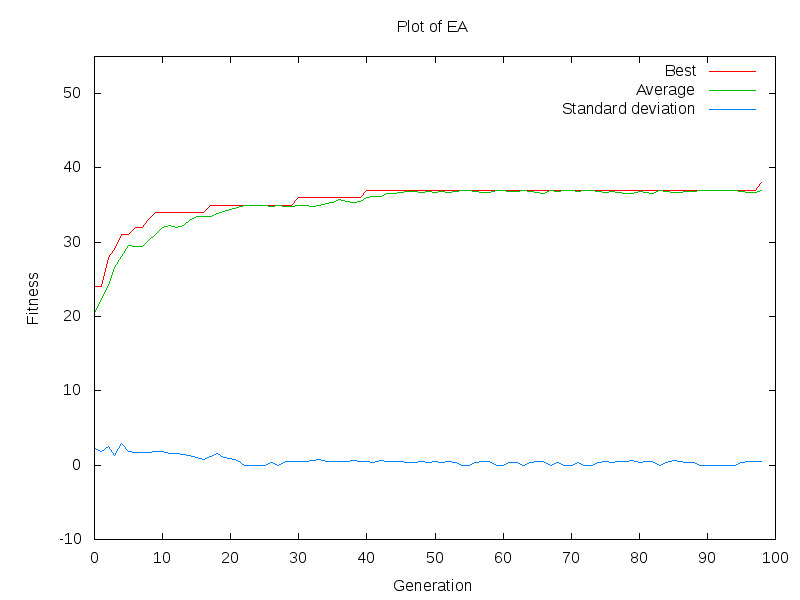
\includegraphics[width=0.49\textwidth]{images/21.png}}
\mbox{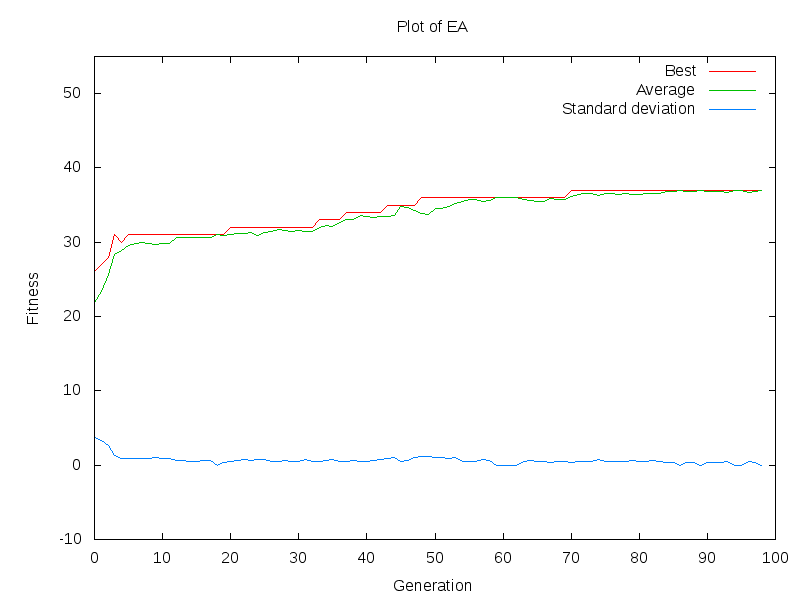
\includegraphics[width=0.49\textwidth]{images/22.png}}
\end{center}
\caption{Plotting of two EA runs:
Size of child pool: 7,
Size of adult pool: 7,
number of generations: 99,
mutation rate: 0.1,
crossover rate: 0.9,
selection protocol: Full generational replacement,
selection strategy: Fitness proportionate,
elitism: 2}
\label{fig:2}
\end{figure}

Changing the mutation rate to 0.1 and the crossover rate to 0.9 resulted in no solution
being found within 100 generations. See figure \ref{fig:2}.

\begin{figure}[ht]
\begin{center}
\mbox{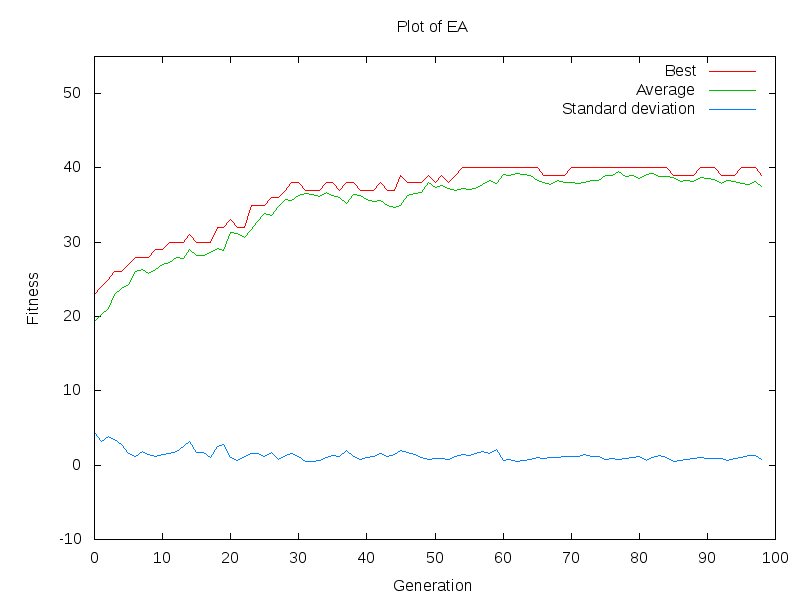
\includegraphics[width=0.49\textwidth]{images/31.png}}
\mbox{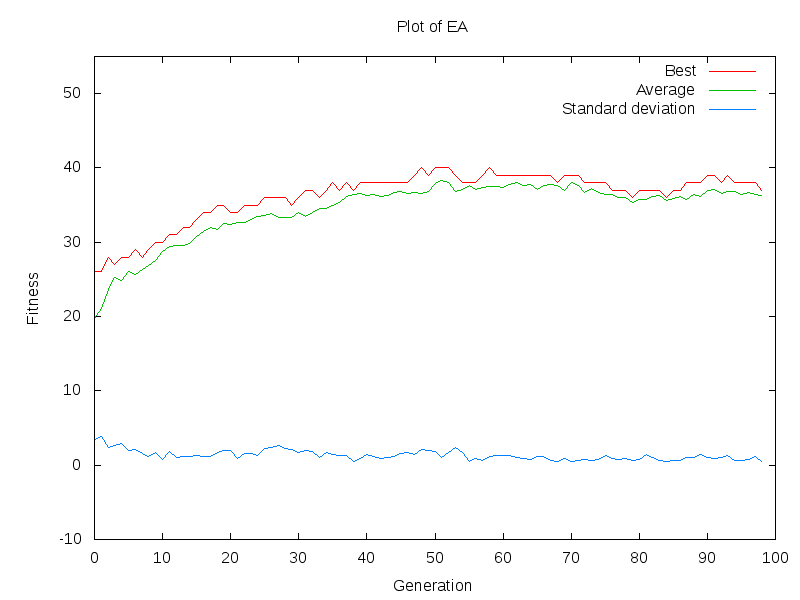
\includegraphics[width=0.49\textwidth]{images/32.png}}
\end{center}
\caption{Plotting of two EA runs:
Size of child pool: 7,
Size of adult pool: 7,
number of generations: 99,
mutation rate: 0.6,
crossover rate: 0.3,
selection protocol: Full generational replacement,
selection strategy: Fitness proportionate,
elitism: 2}
\label{fig:3}
\end{figure}

Changing the mutation rate to 0.6 and the crossover rate to 0.3 resulted in a solution
beeing found (See figure \ref{fig:3},) but not as early and not as consistently.

\begin{figure}[ht]
\begin{center}
\mbox{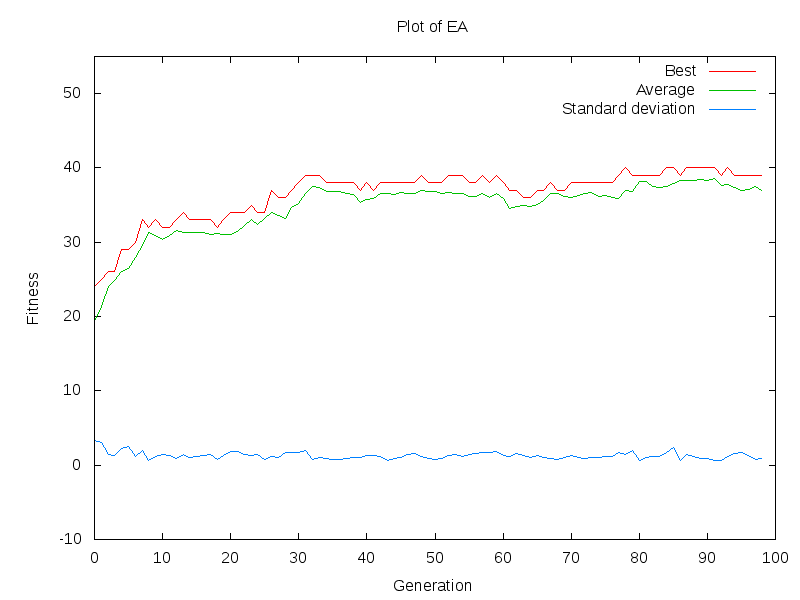
\includegraphics[width=0.49\textwidth]{images/41.png}}
\mbox{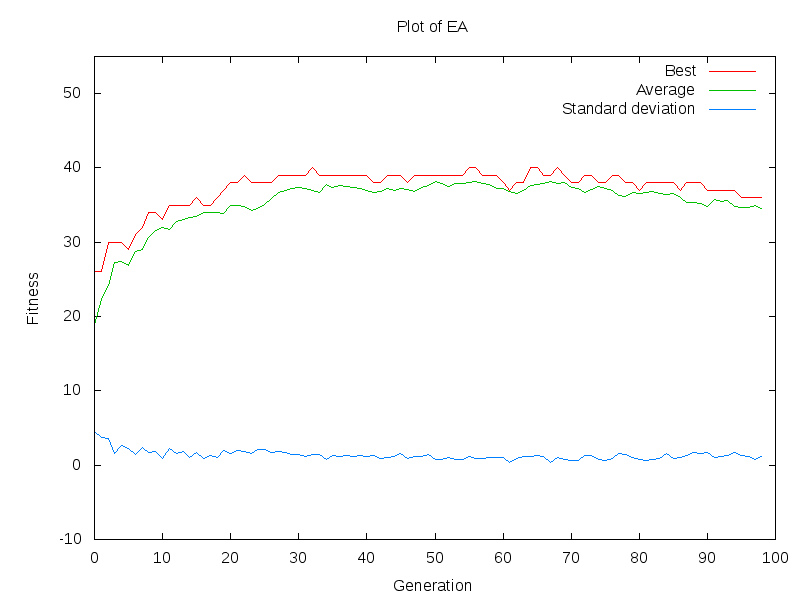
\includegraphics[width=0.49\textwidth]{images/42.png}}
\end{center}
\caption{Plotting of two EA runs:
Size of child pool: 7,
Size of adult pool: 7,
number of generations: 99,
mutation rate: 0.8,
crossover rate: 0.2,
selection protocol: Full generational replacement,
selection strategy: Fitness proportionate,
elitism: 2}
\label{fig:4}
\end{figure}
Changing the mutation rate to 0.8 and the crossover rate to 0.2 resulted in a solution
beeing found (See figure \ref{fig:4},) but not as early and not as consistently.

\subsection*{Parent selection experiment} %4. Using the best-found population-size, mutation and crossover settings from the previous experiments, do a new set of experiments to find the parent selection mechanism that gives the best results. Again, document your experiments with fitness plots. (2 points).

\begin{figure}[ht]
\begin{center}
\mbox{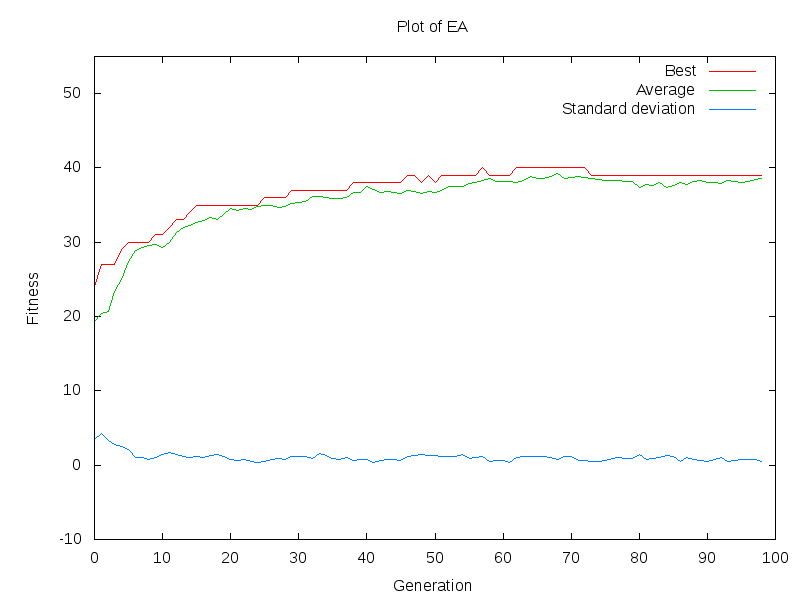
\includegraphics[width=0.49\textwidth]{images/fit1.png}}
\mbox{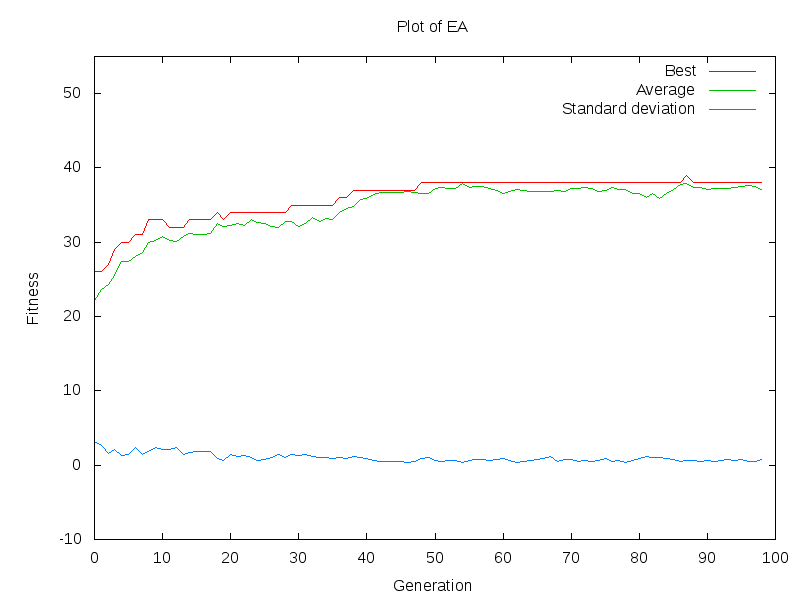
\includegraphics[width=0.49\textwidth]{images/fit2.png}}
\end{center}
\caption{Plotting of two EA runs:
Size of child pool: 7,
Size of adult pool: 7,
number of generations: 99,
mutation rate: 0.3,
crossover rate: 0.6,
selection protocol: Full generational replacement,
selection strategy: Fitness proportionate,
elitism: 2}
\label{fig:5}
\end{figure}


\begin{figure}[ht]
\begin{center}
\mbox{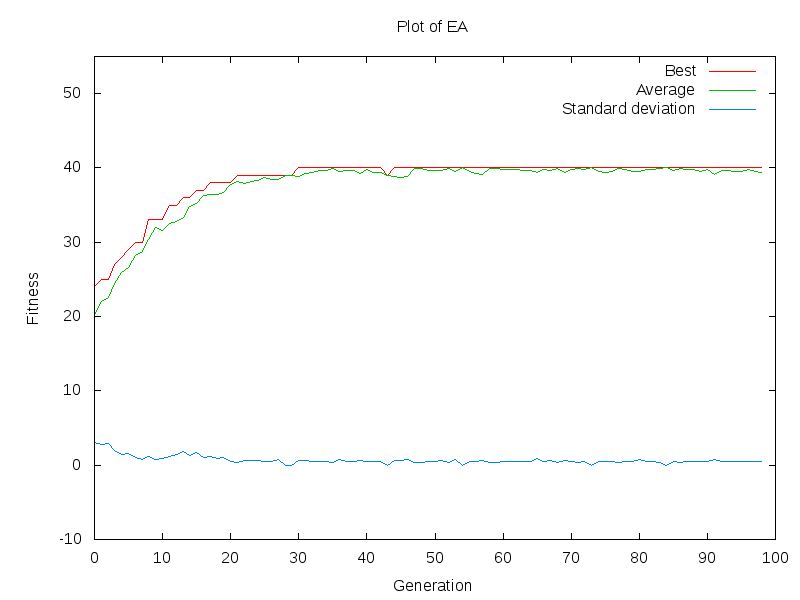
\includegraphics[width=0.49\textwidth]{images/sig1.png}}
\mbox{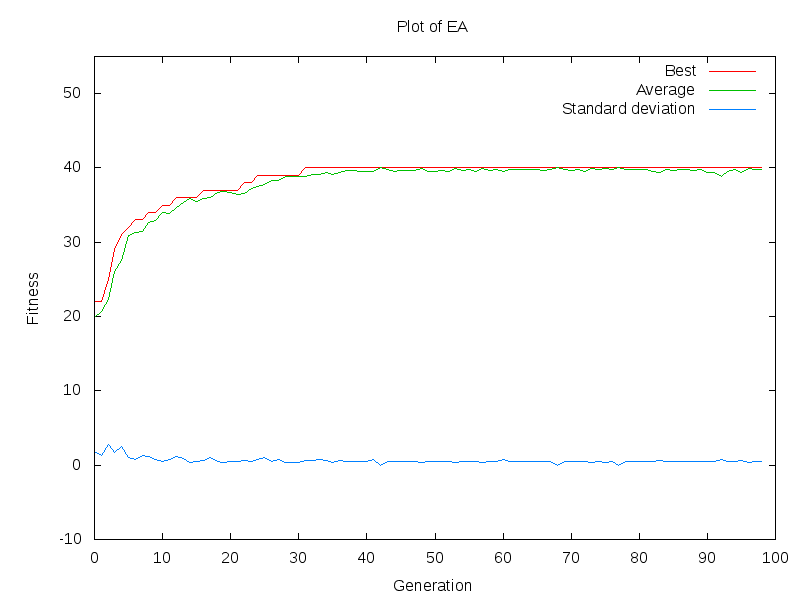
\includegraphics[width=0.49\textwidth]{images/sig2.png}}
\end{center}
\caption{Plotting of two EA runs:
Size of child pool: 7,
Size of adult pool: 7,
number of generations: 99,
mutation rate: 0.3,
crossover rate: 0.6,
selection protocol: Full generational replacement,
selection strategy: Sigma Scaling,
elitism: 2}
\label{fig:6}
\end{figure}

Sigma scaling obviosly cause the population to converge faster.

\begin{figure}[ht]
\begin{center}
\mbox{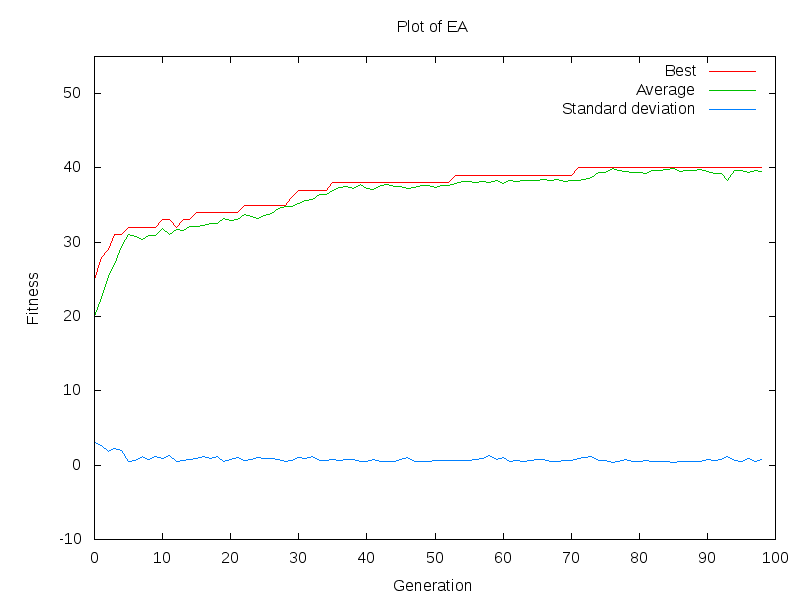
\includegraphics[width=0.49\textwidth]{images/bol1.png}}
\mbox{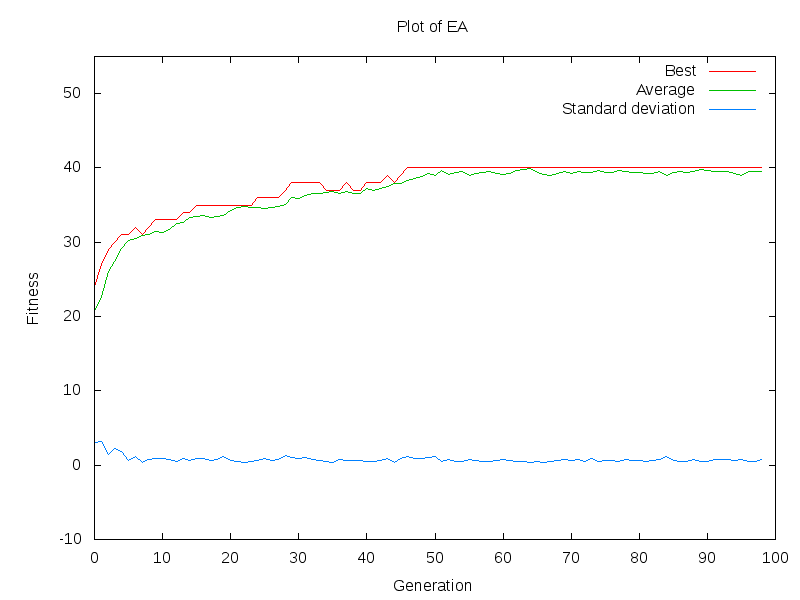
\includegraphics[width=0.49\textwidth]{images/bol2.png}}
\end{center}
\caption{Plotting of two EA runs:
Size of child pool: 7,
Size of adult pool: 7,
number of generations: 99,
mutation rate: 0.3,
crossover rate: 0.6,
selection protocol: Full generational replacement,
selection strategy: Boltzmann selection,
elitism: 2,
Temperature: 2}
\label{fig:7}
\end{figure}

Boltzmann scaling does not scale as fast as sigma scaling, but faster than
fitness proportionate.

\begin{figure}[ht]
\begin{center}
\mbox{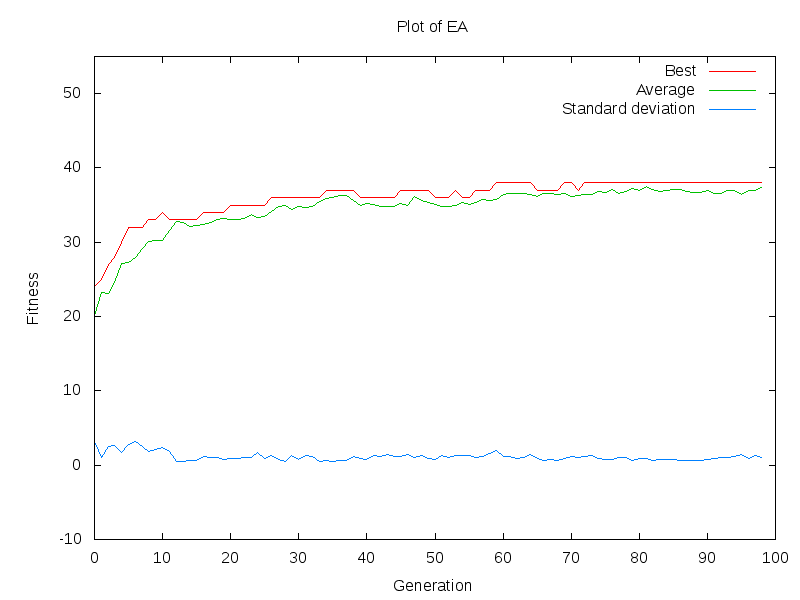
\includegraphics[width=0.49\textwidth]{images/ran1.png}}
\mbox{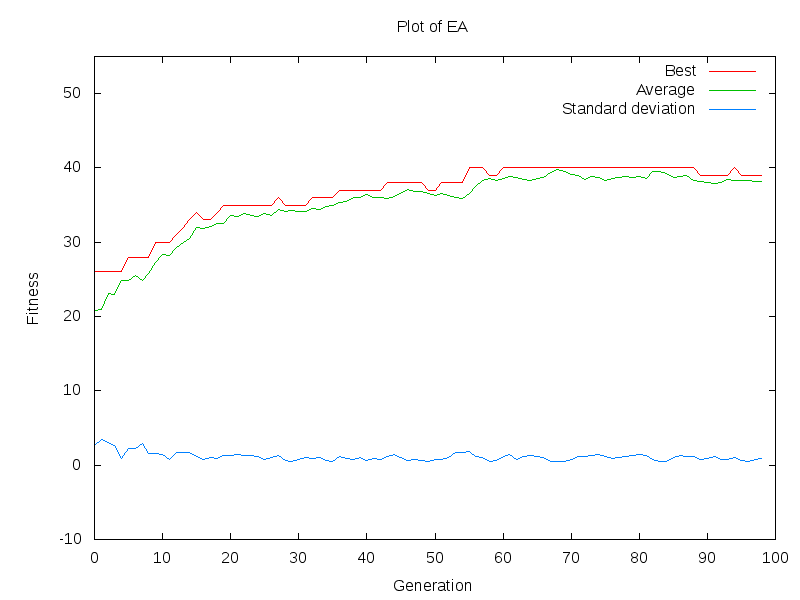
\includegraphics[width=0.49\textwidth]{images/ran2.png}}
\end{center}
\caption{Plotting of two EA runs:
Size of child pool: 7,
Size of adult pool: 7,
number of generations: 99,
mutation rate: 0.3,
crossover rate: 0.6,
selection protocol: Full generational replacement,
selection strategy: Rank Selection,
elitism: 2}
\label{fig:8}
\end{figure}


\begin{figure}[ht]
\begin{center}
\mbox{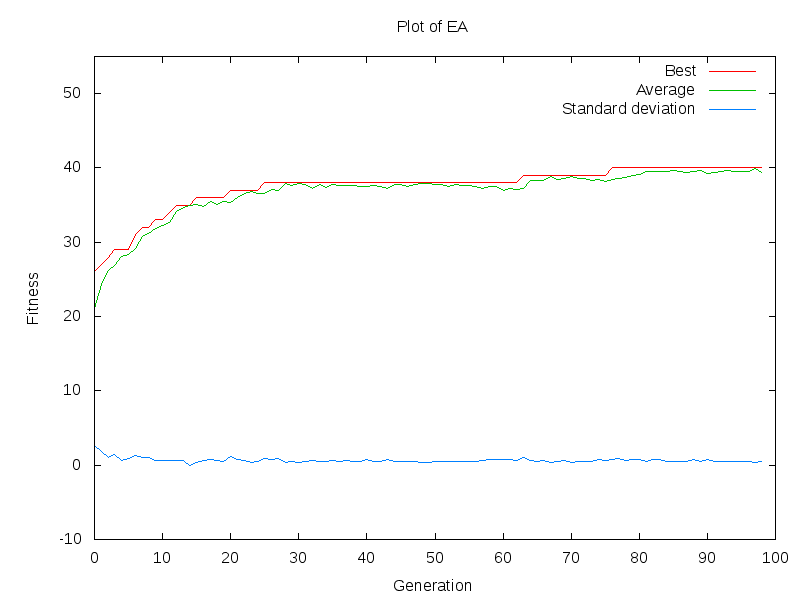
\includegraphics[width=0.49\textwidth]{images/tou1.png}}
\mbox{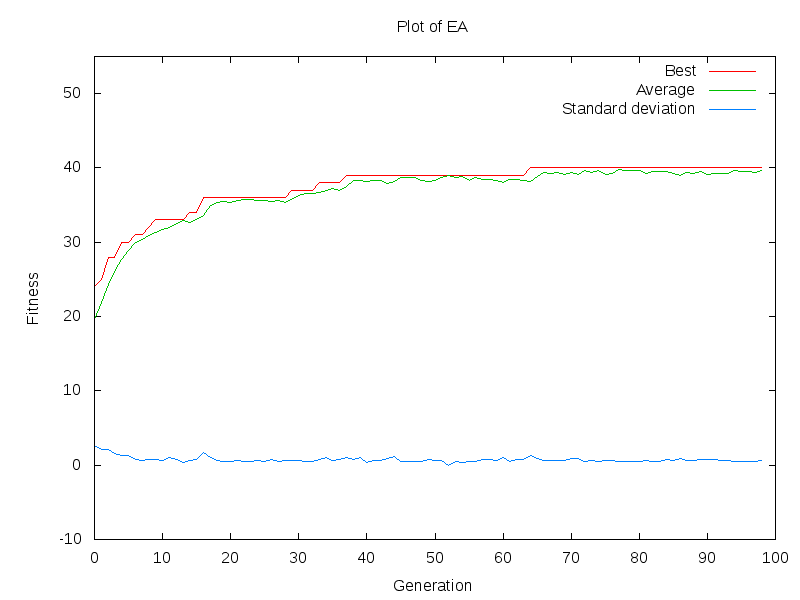
\includegraphics[width=0.49\textwidth]{images/tou2.png}}
\end{center}
\caption{Plotting of two EA runs:
Size of child pool: 7,
Size of adult pool: 7,
number of generations: 99,
mutation rate: 0.3,
crossover rate: 0.6,
selection protocol: Full generational replacement,
selection strategy: Tournament selection,
elitism: 2,
Tournament size: 3}
\label{fig:8}
\end{figure}


\subsection*{Random bit vector} %5. Modify the target bit string from all 1’s to a random bit vector of length 40. Do you expect this to increase the difficulty of the problem? Run the EA and find out. Document your results from at least 4 different runs as part of your comparison. Explain the results. (2 points).


\end{document}
